\section{Outlook and guidance for future separators}

\subsection{Recoil separators planned and under construction}
\subsubsection{St. George -- Notre Dame}

St. George (Strong Gradient Electromagnetic Online Recoil separator for capture Gamma Ray Experiments) \cite{cou08} is a recoil separator under construction at the Institute for Structure and Nuclear Astrophysics at the University of Notre Dame. The design is optimized for the study of astrophysical low energy ($\alpha,\gamma$) reactions for up to A=40 beam mass. The beams will be provided by the new 5MV accelerator at the laboratory. The separator has design acceptance values of $\pm$40 mrad in angle and $\pm$7.5\% in energy. It is built in a configuration providing selection of a single charge state via magnetic analysis, before mass separation is performed in a Wien filter (see figure \ref{fig:stgeorge}), with a final resolving power of $m/\Delta m=100$. It is designed to have high a beam suppression factor of $\ge10^{15}$. In particular the Wien filter element of this separator is specially optimized to improve the filtering efficiency, achieved by minimizing the magnetic dipole component fringe fields and by incorporating specially-shaped electrodes so that the electric fringe fields closely follow the magnetic ones. 

\begin{figure}
\resizebox{0.9\columnwidth}{!}{
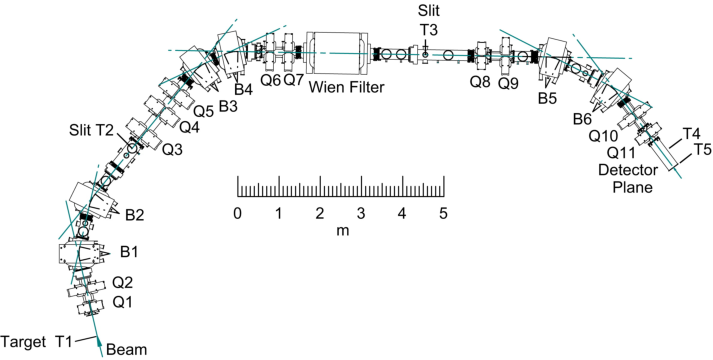
\includegraphics{stgeorge}
}
%\vspace{5cm}       % Give the correct figure height in cm
\caption{Schematic view of the St. George separator. Taken from \cite{cou08}.}
\label{fig:stgeorge}
\end{figure}

\subsubsection{KRS -- KoRIA}
\subsubsection{SECAR -- FRIB}

\subsection{Suggested avenues of technical development} 
